\subsection{Ny løsning}
Konstruksjonen har blitt laget og testet. I dette kapittelet vises bilder av den endelige ramme konstruksjonen samt data fra testing av rammen. 
Testingen ble i hovedsak utført ved å legge last på rammen. Det er i utgangspunktet vanskelig å beregne makslast på gammelt treverk. Dette på grunn av at det er vanskelig å anslå hvor skadet treverket er. Det er observert mange hull og skader i treverket på grunn av tidligere montering og bruk. Dette i kombinasjon med usikkerheten rundt fukt hvor nedbrutt treverket er, gjør dimensjonering og fastsettelse av styrkeegenskaper vanskelig.
Testingen som nevnt utført ved å laste rammen så mye som det var forsvarlig utifra et subjektivt synspunkt. De ble under testing lastet om i overkant av 200 kg på rammen. Dette blir derfor maks last på rammen. Videre er det av rammens dimensjoner gitt en maksimal lastlengde 3000 mm, en maksimal lastebredde på 1500 mm samt en maksimal lastehøyde på 1300 mm.
Bildene fra den endelige konstruksjonen er vist under     
\begin{figure}[H]
\centering   
\subfloat[Rammen]{\includegraphics[width=0.5\textwidth]{images/NL1.JPG}}
\subfloat[Rammen på støtteben]{\includegraphics[width=0.5\textwidth]{images/NL2.JPG}}
\caption{Konstruksjonen}
\label{B1}
\end{figure}
\begin{figure}[H]
\centering   
\subfloat[Bakre låsing]{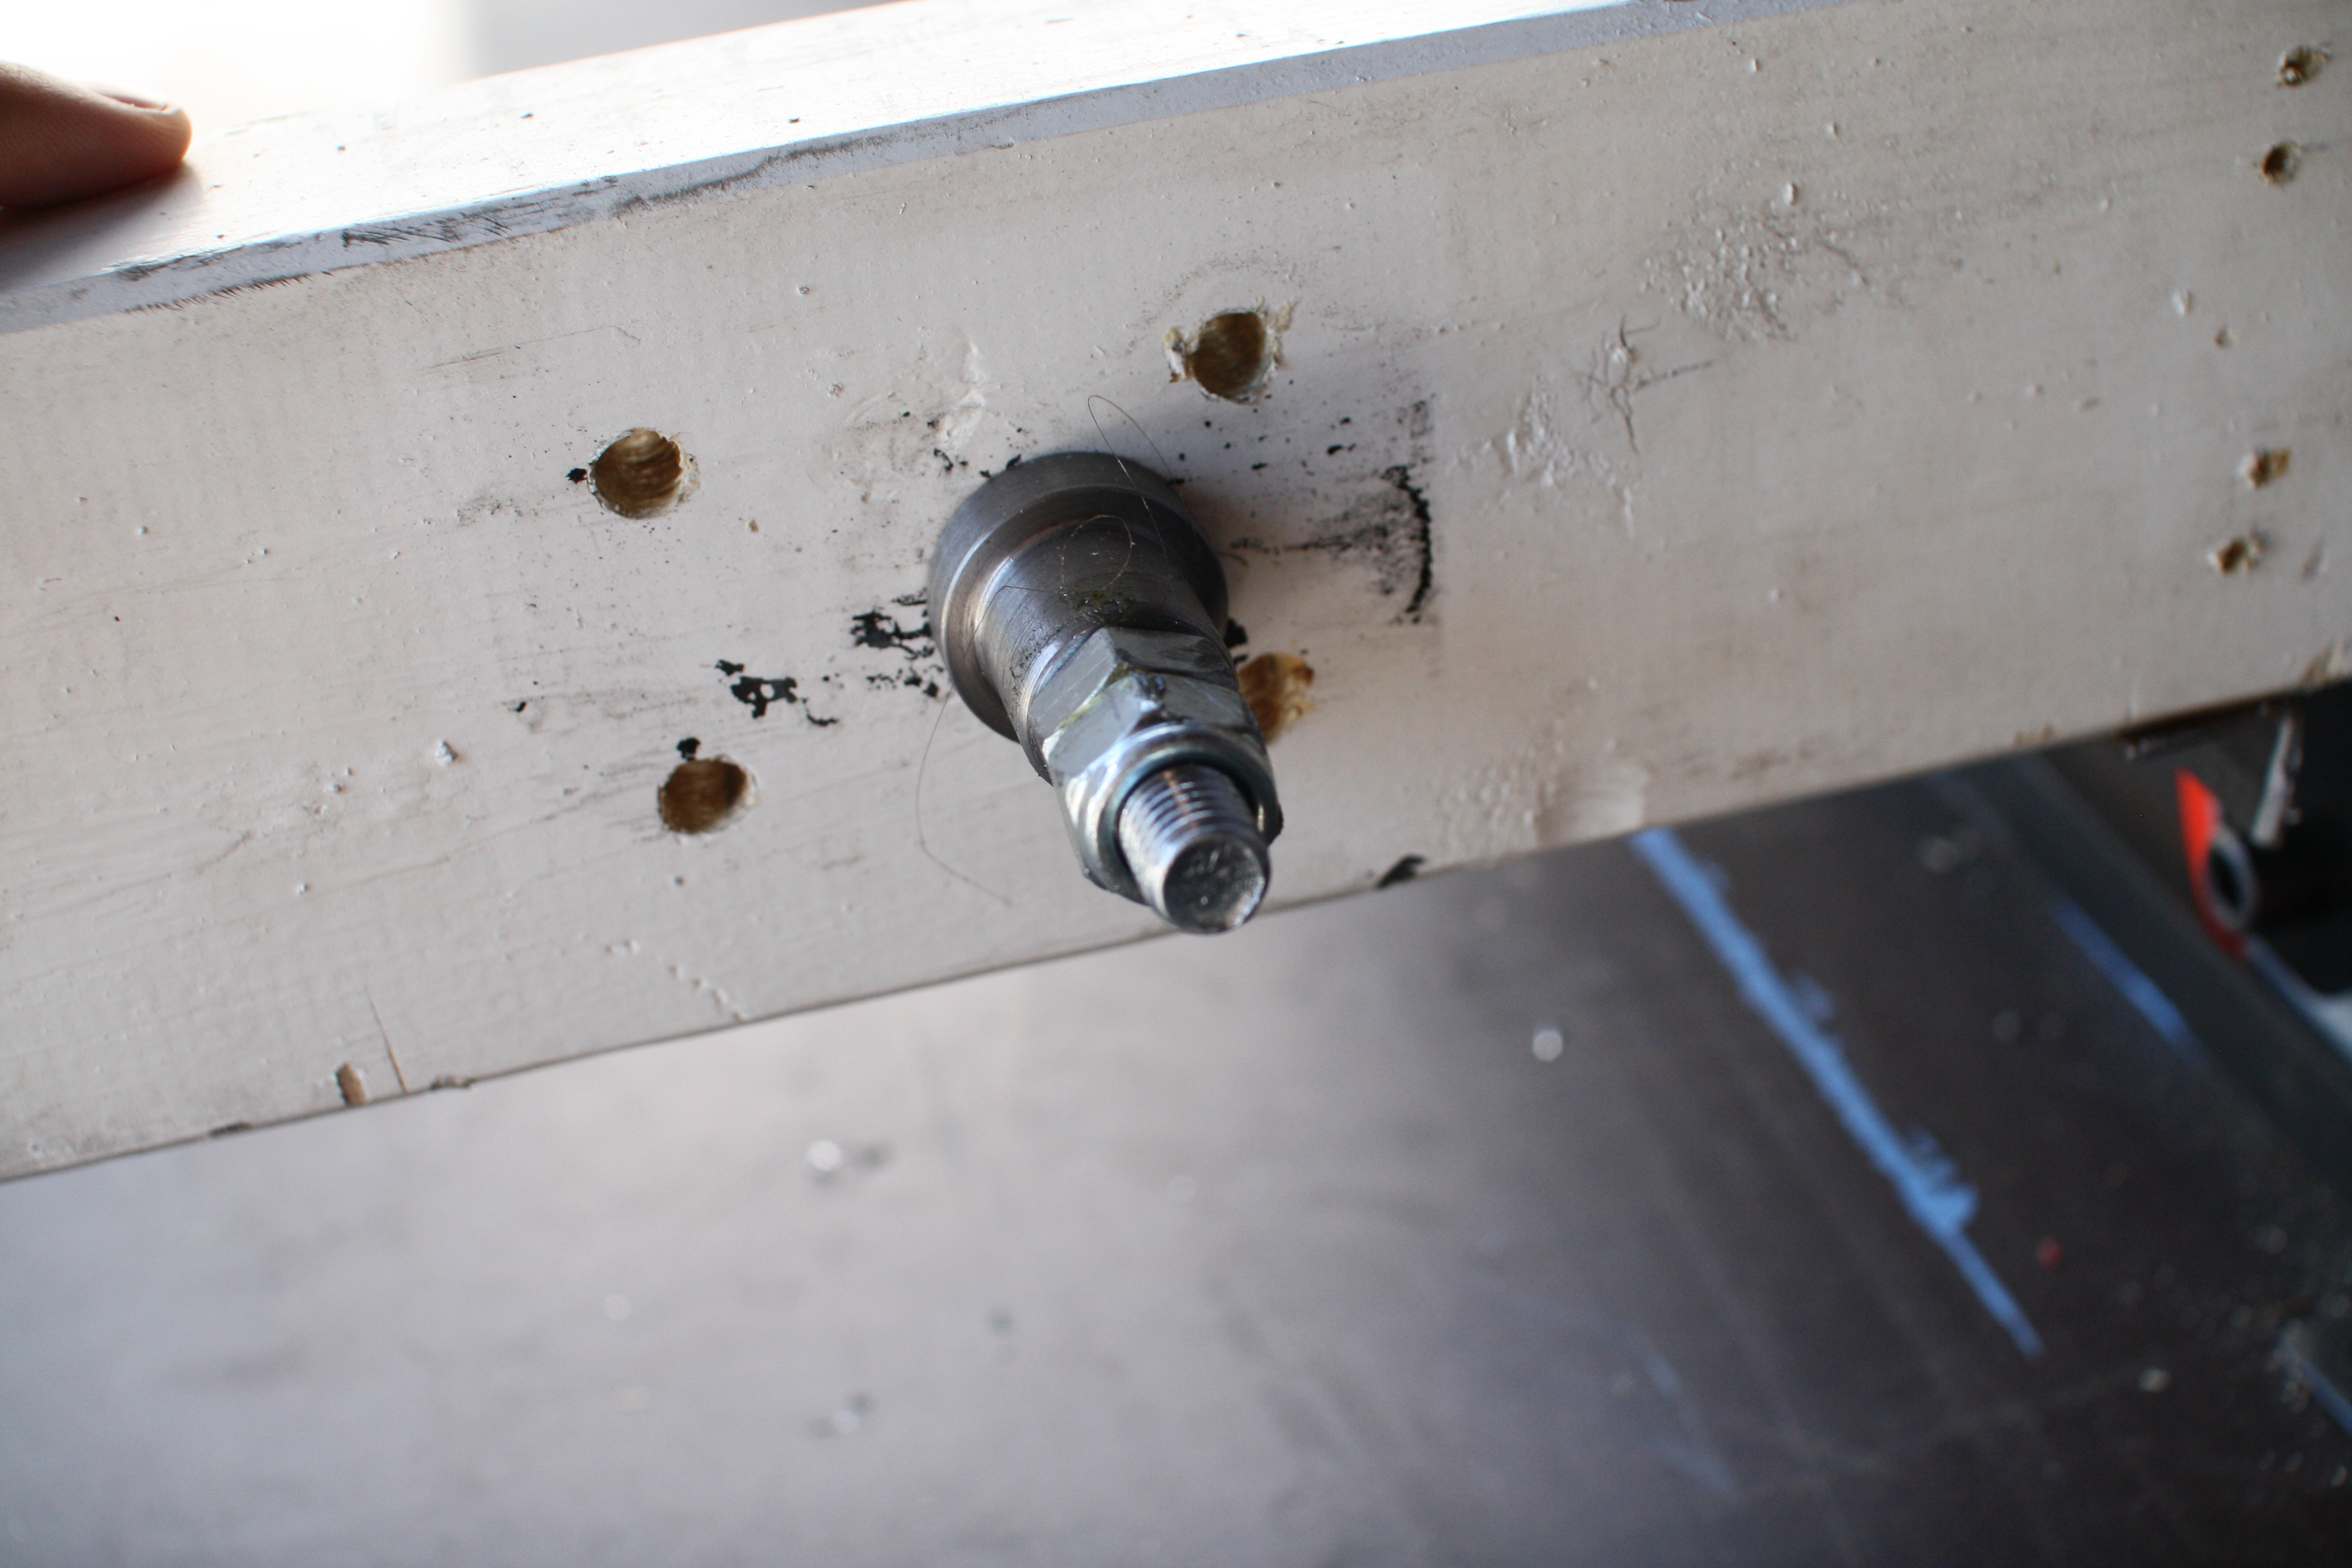
\includegraphics[width=0.45\textwidth]{images/NL3.JPG}}
\subfloat[Bakre låsetapp]{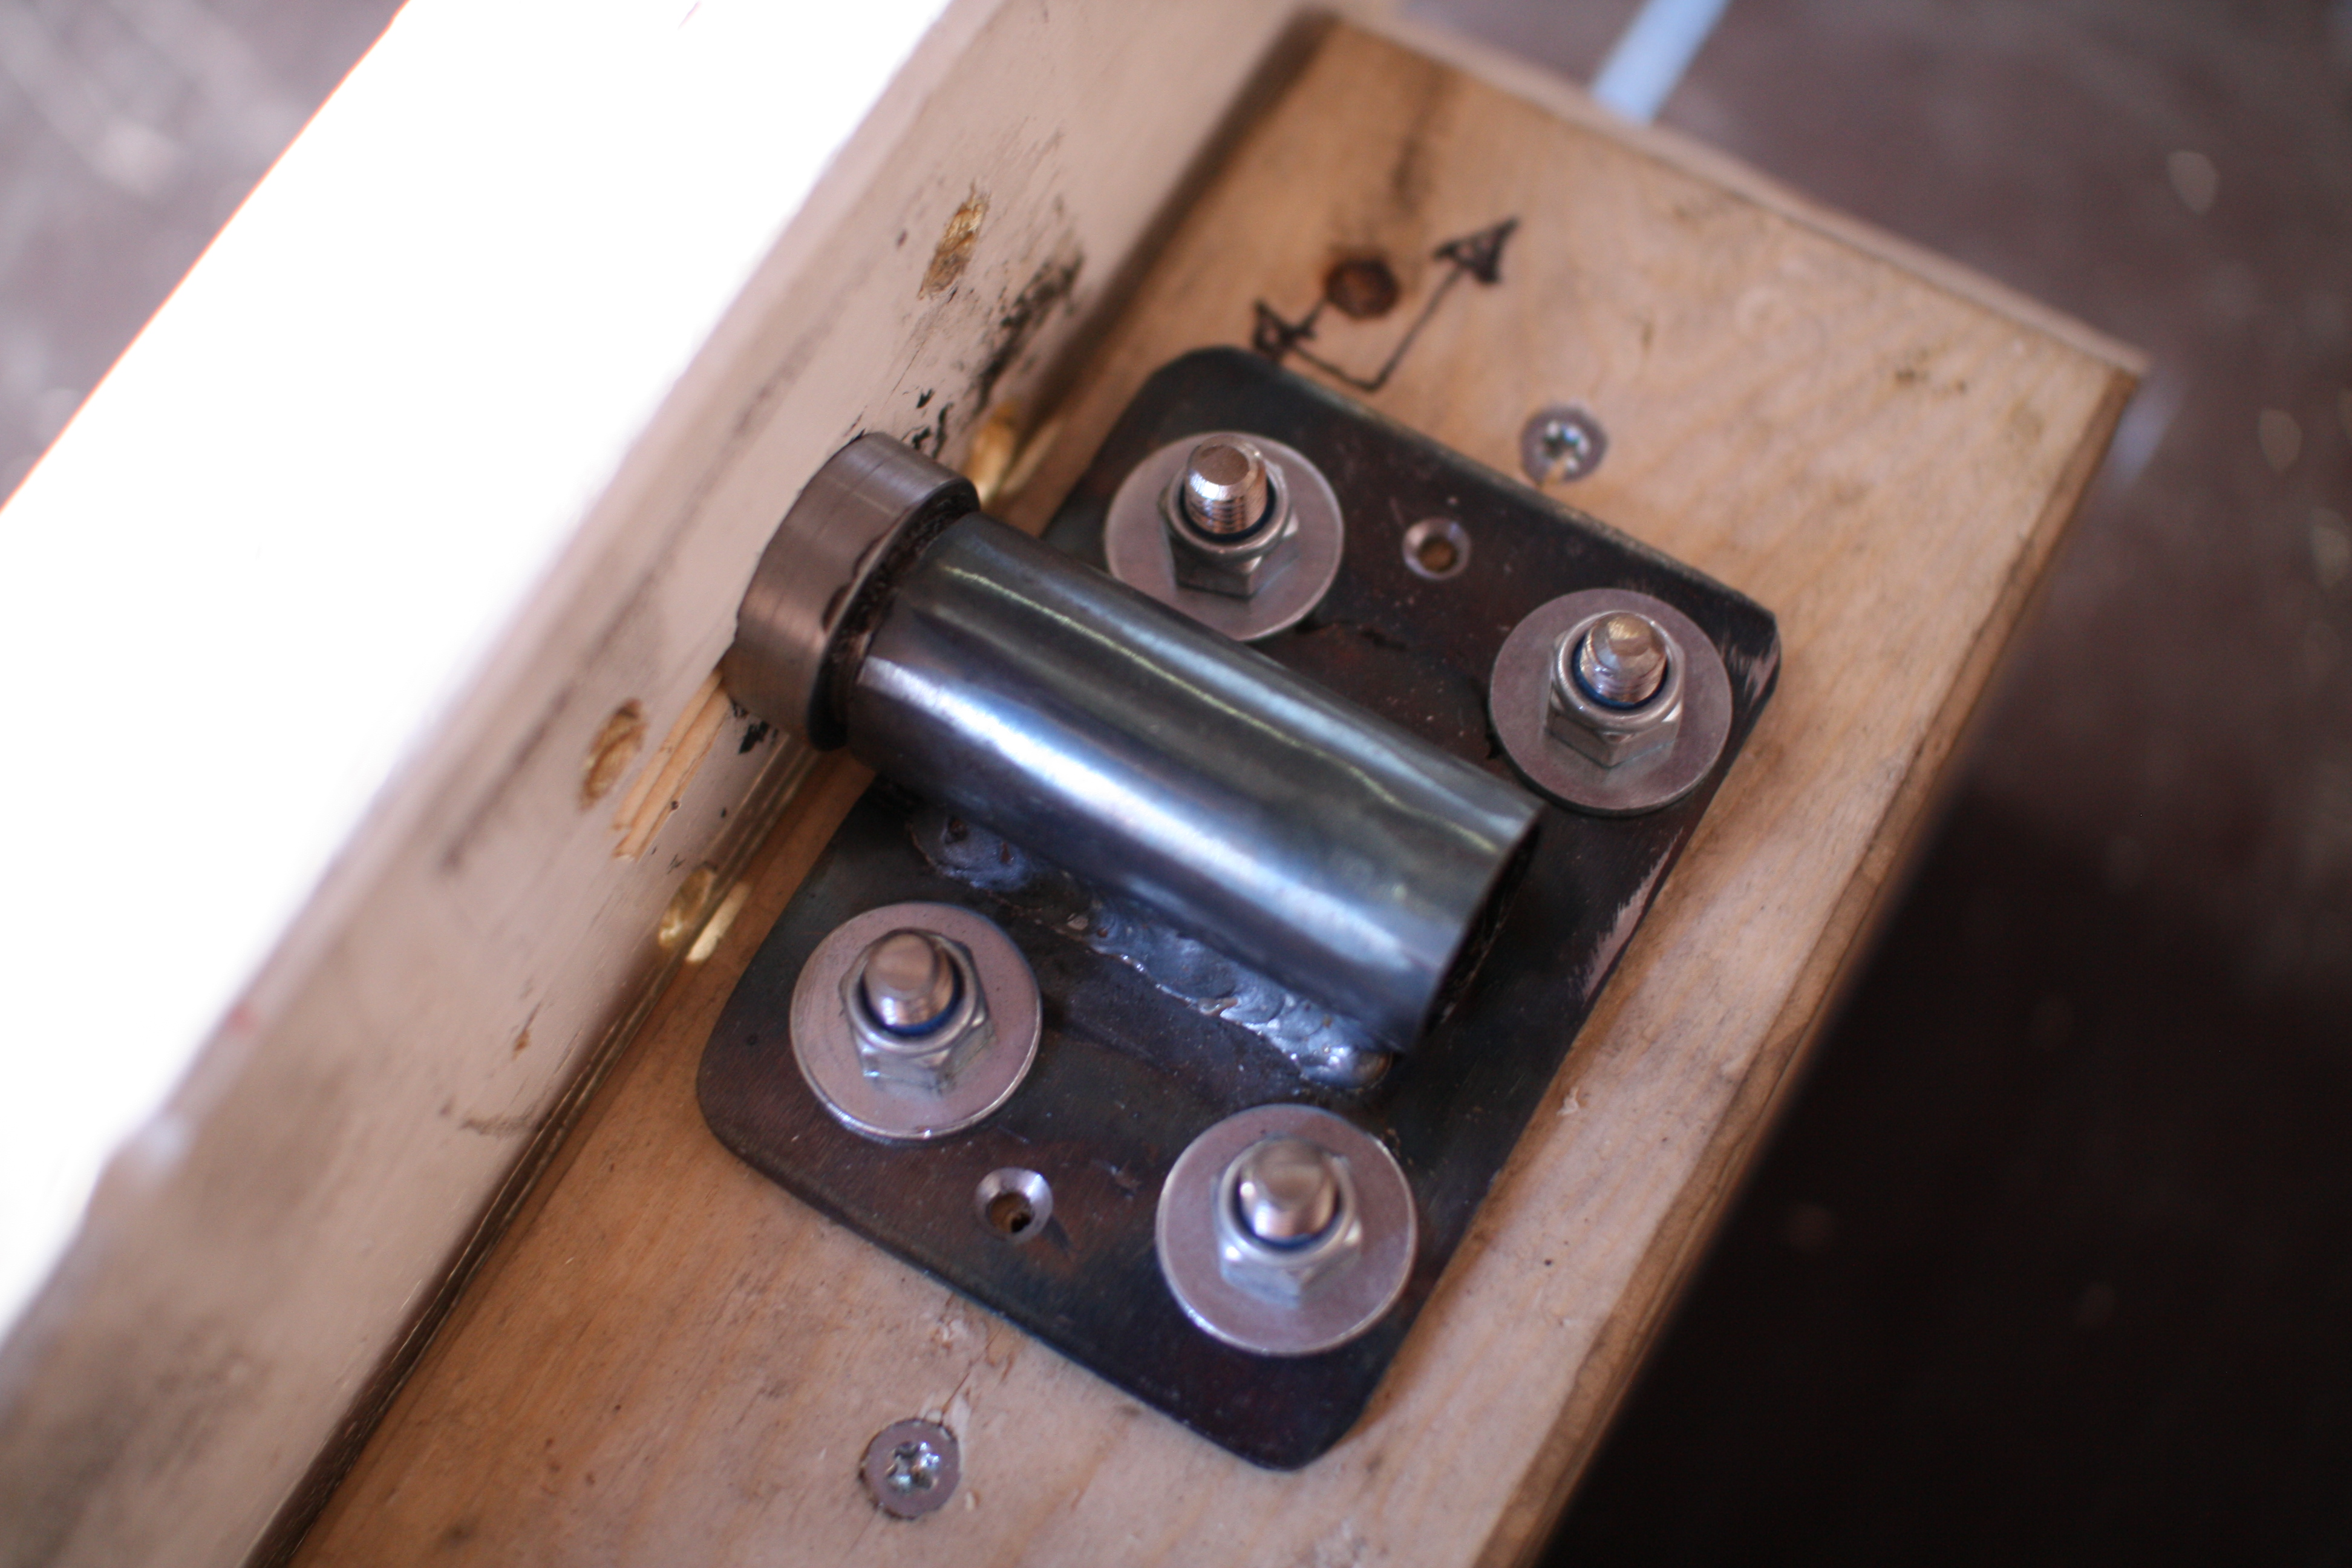
\includegraphics[width=0.45\textwidth]{images/NL4.JPG}}
\caption{Bakre låsing}
\label{B2}
\end{figure}
\begin{figure}[H]
\centering   
\subfloat[Støttebrakett]{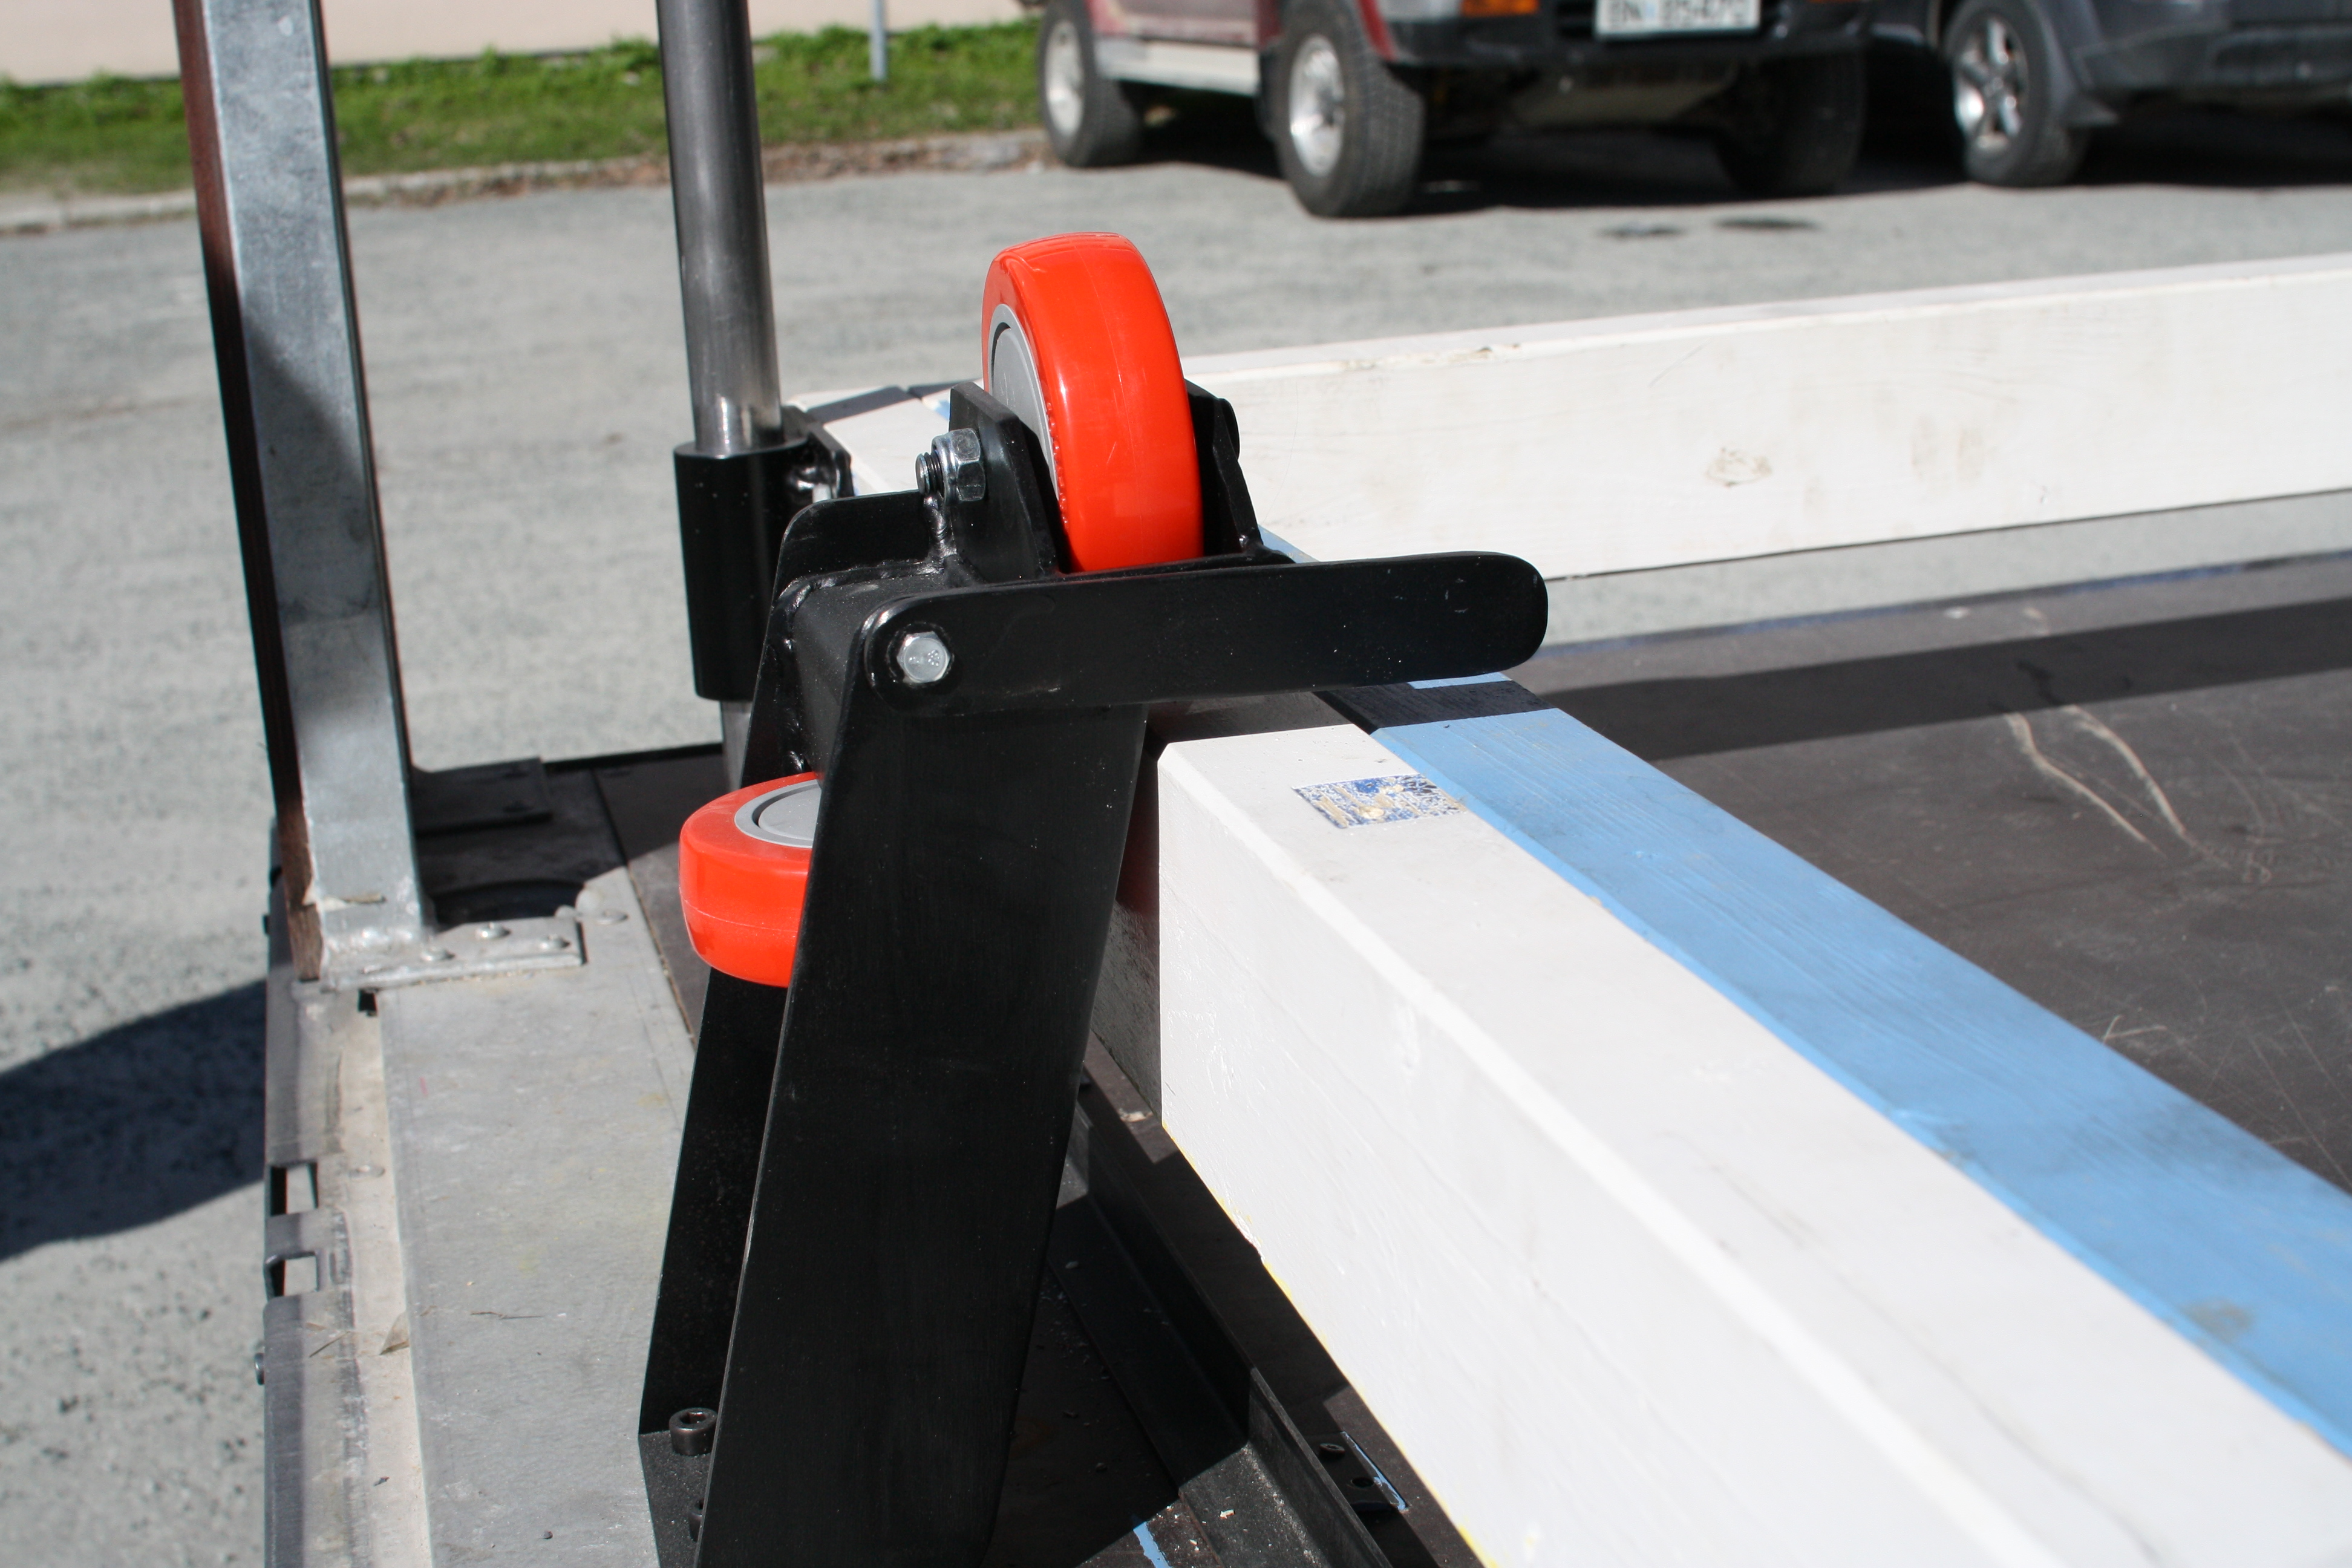
\includegraphics[width=0.45\textwidth]{images/NL5.JPG}}
\subfloat[Idiotsikring]{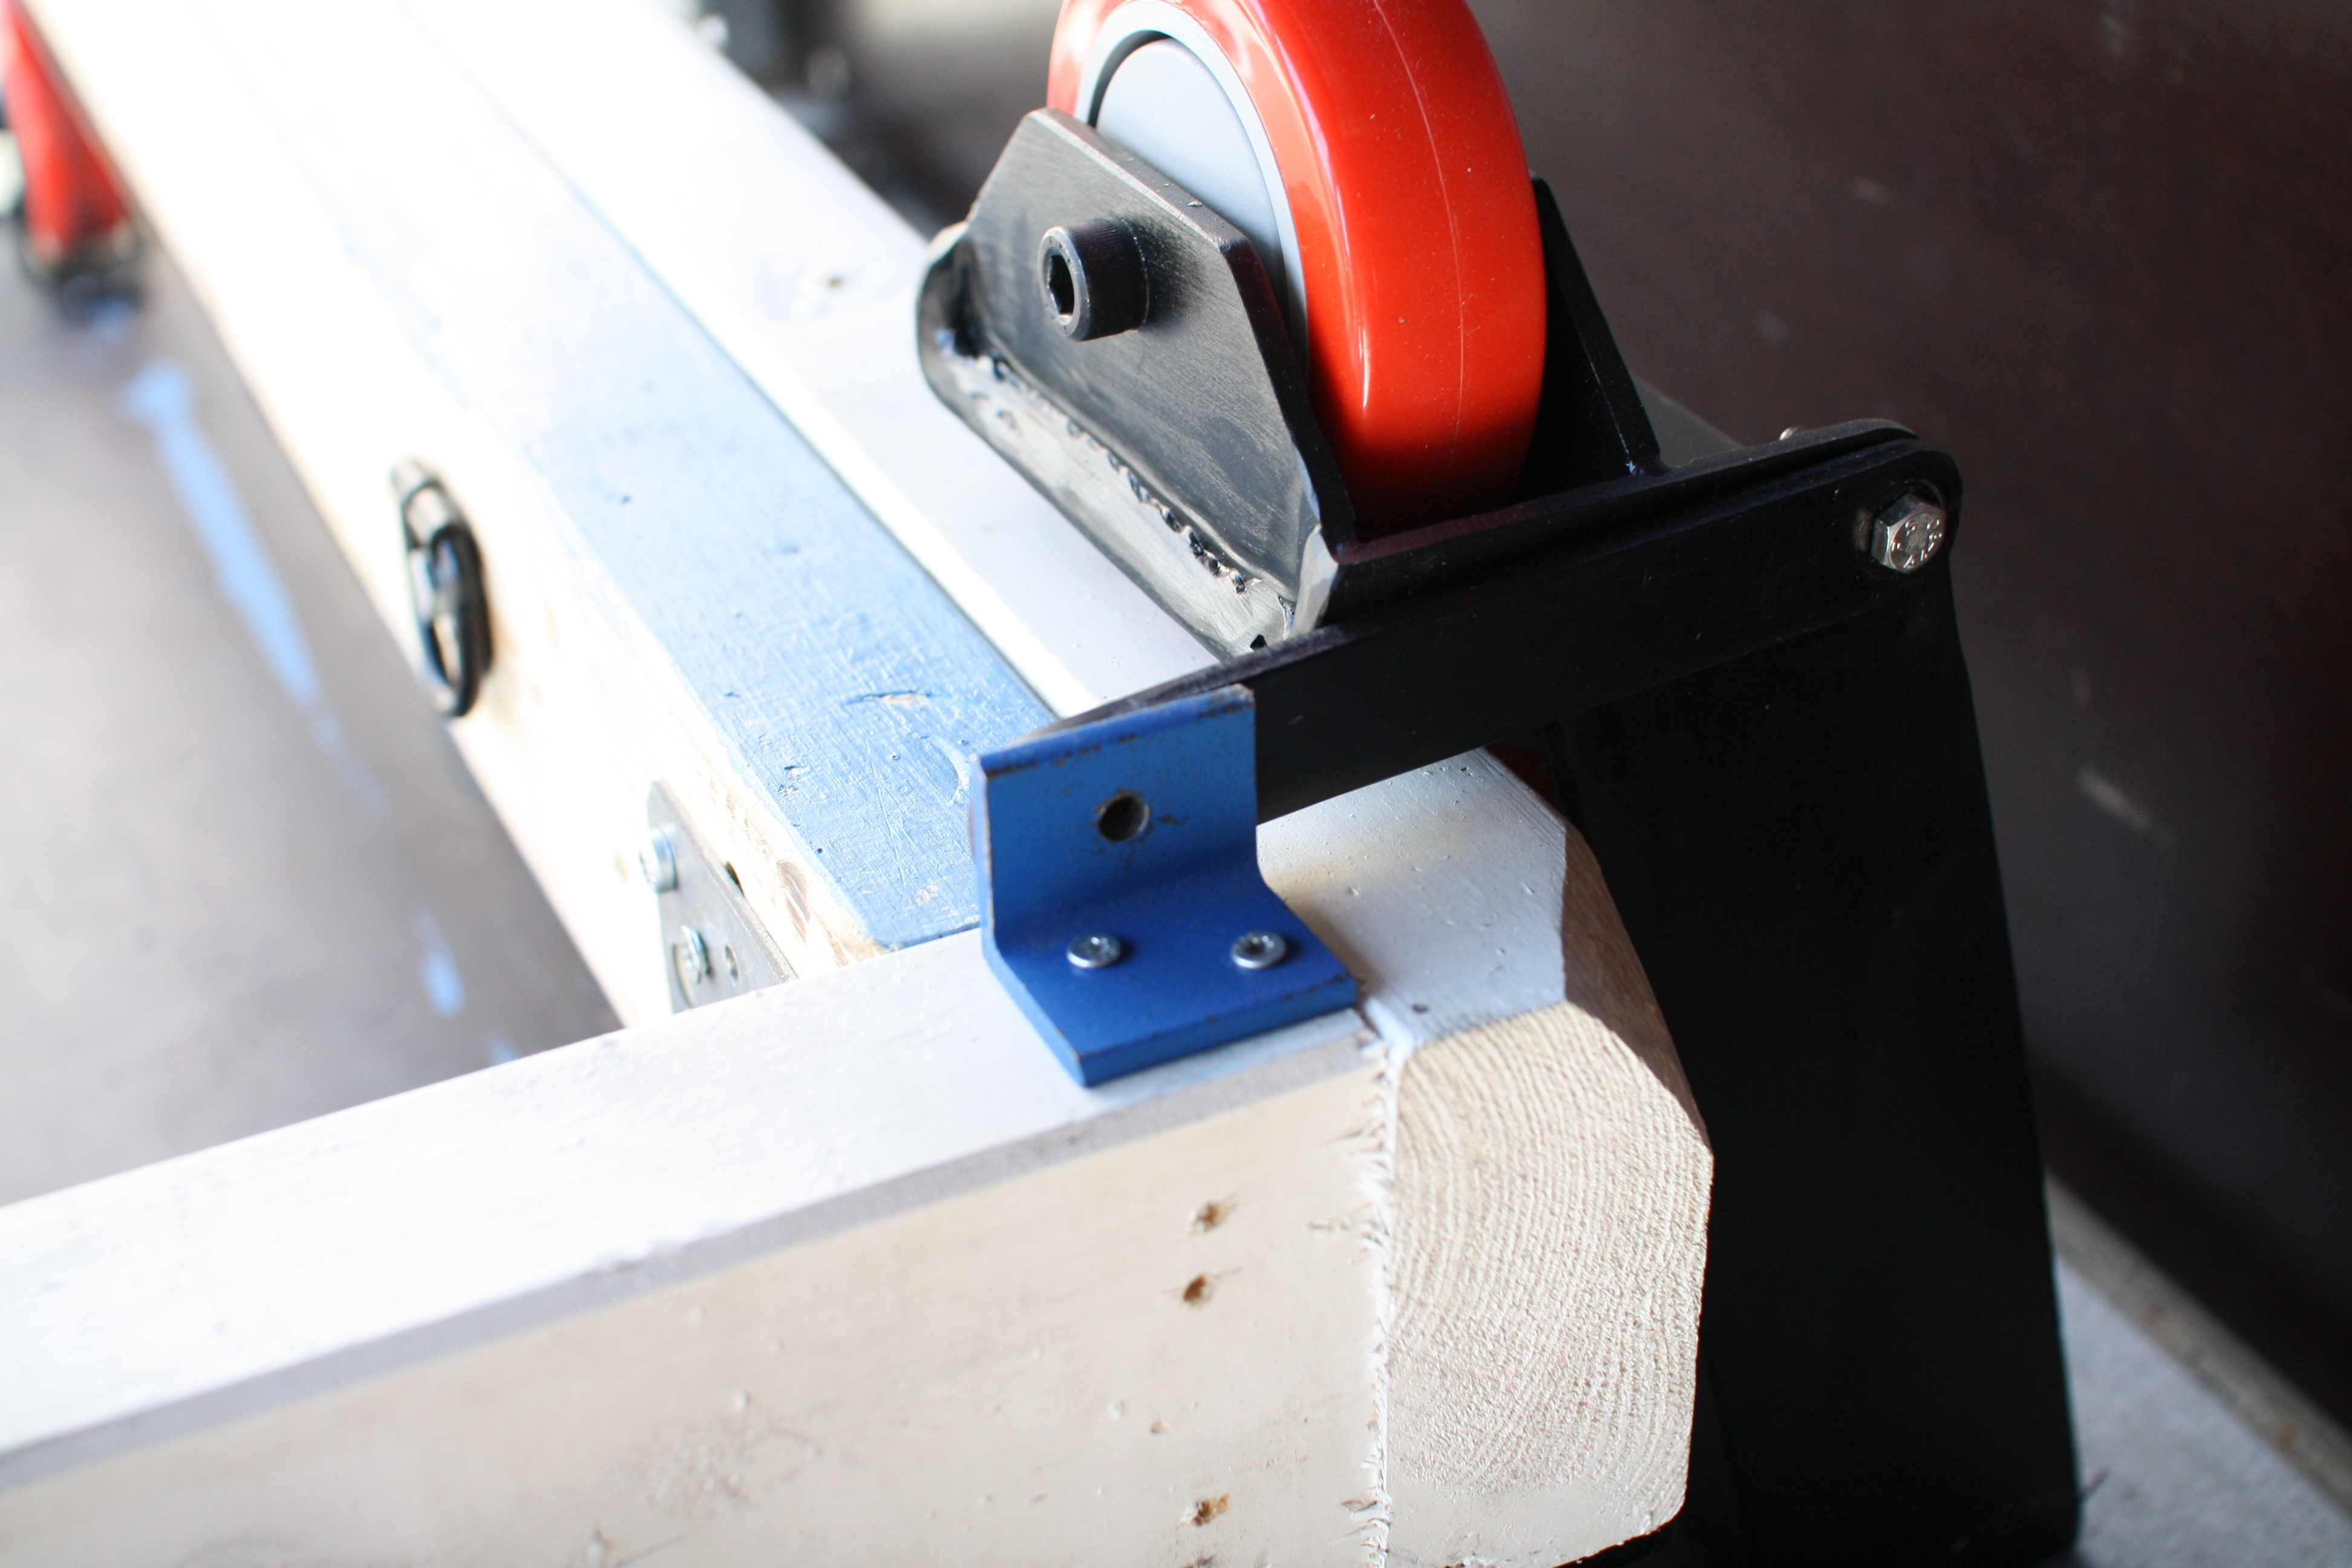
\includegraphics[width=0.45\textwidth]{images/NL6.JPG}}
\caption{Støttebrakett med idiotsikring}
\label{B3}
\end{figure}
\begin{figure}[H]
\centering   
\subfloat[Fremre låsetapp]{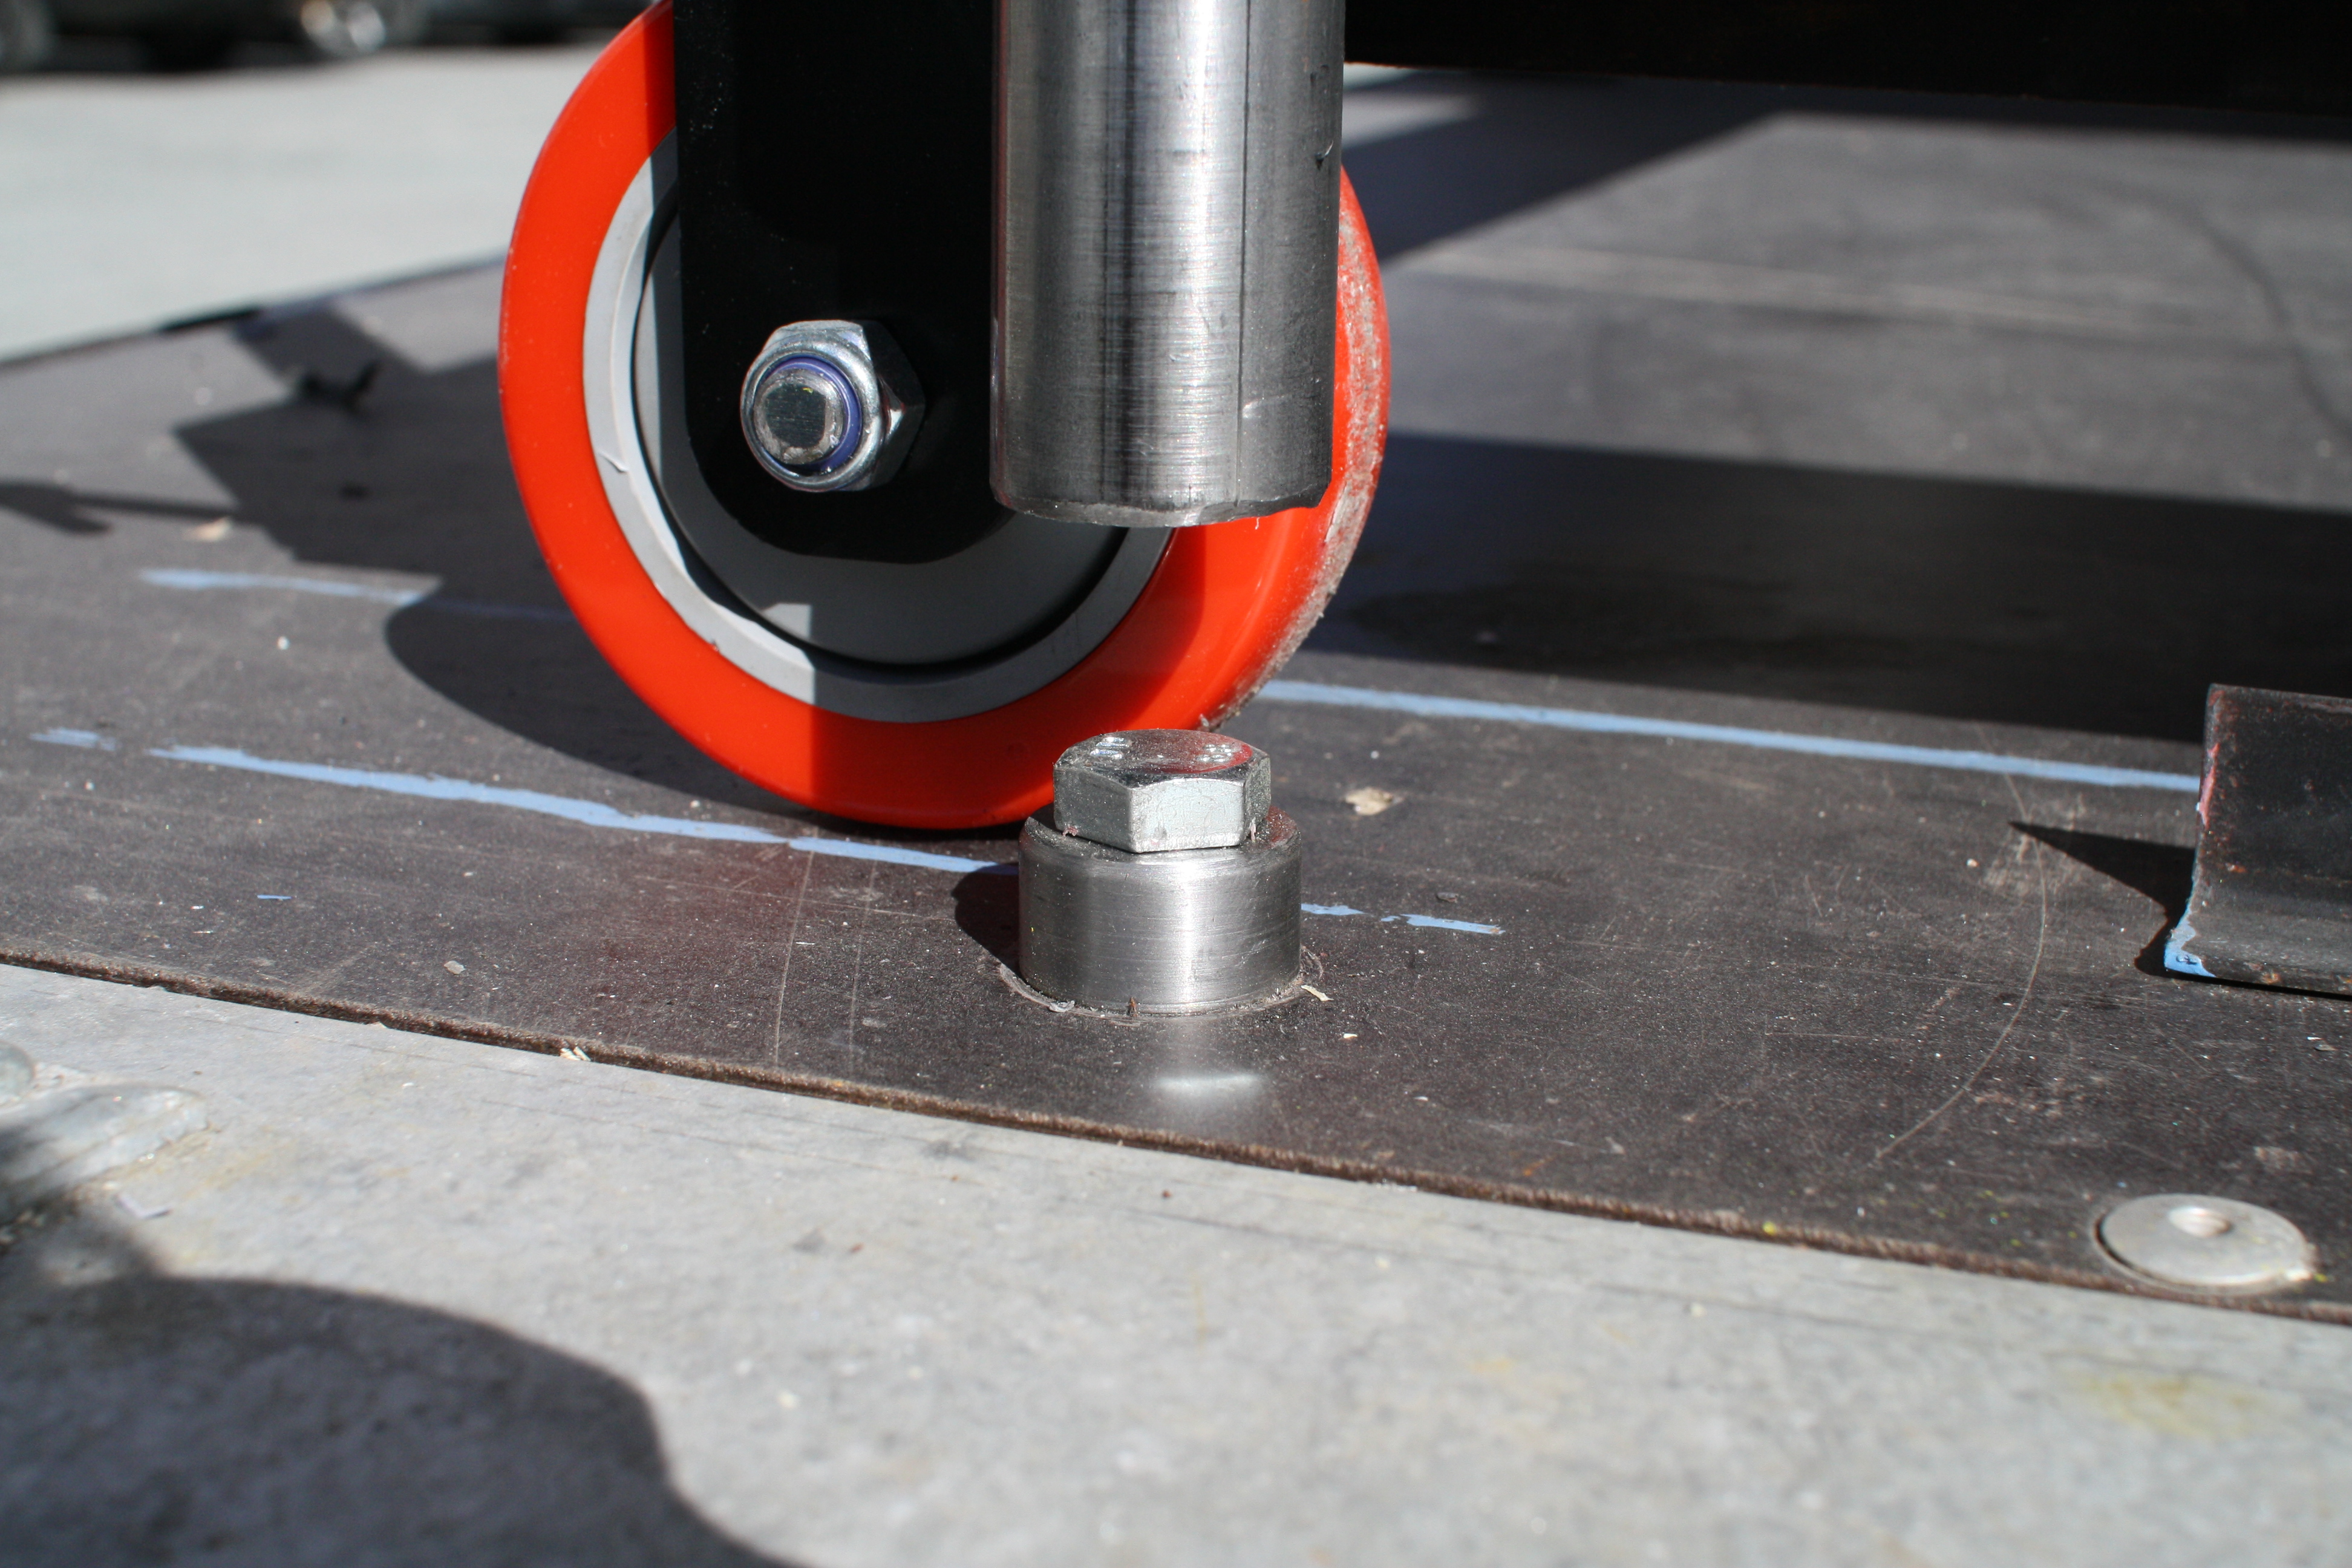
\includegraphics[width=0.45\textwidth]{images/NL7.JPG}}
\subfloat[Fremre låsing]{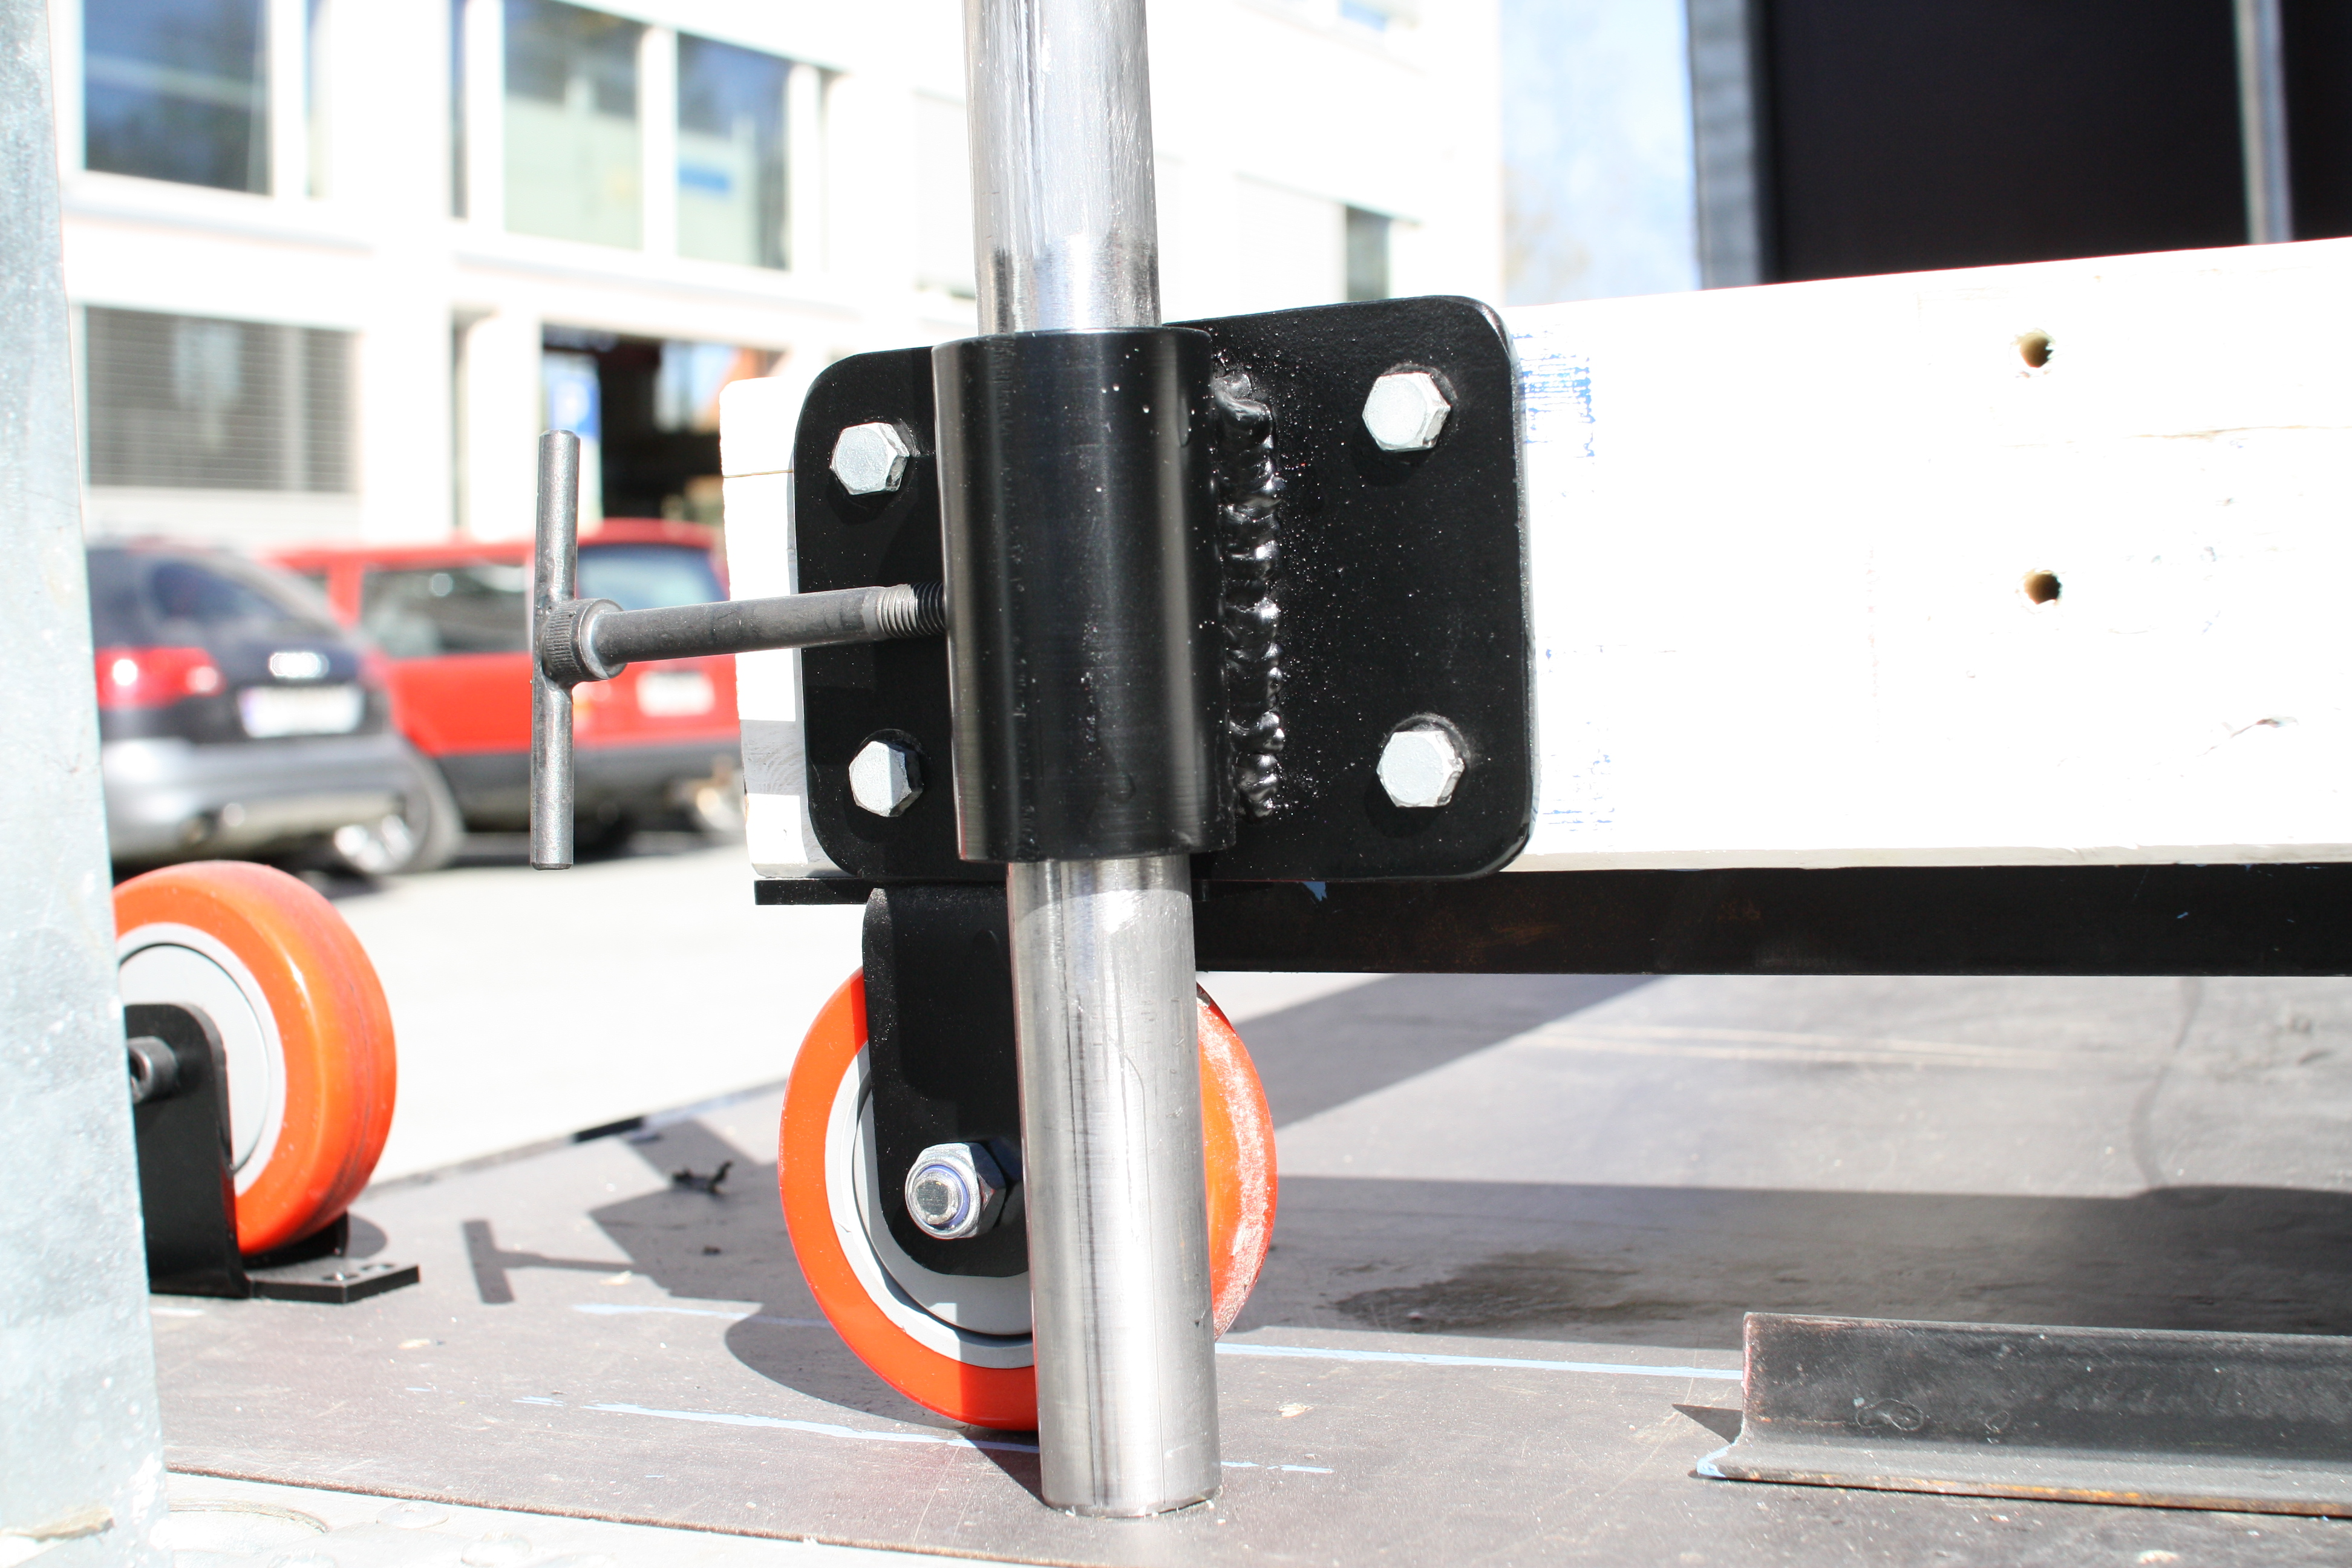
\includegraphics[width=0.45\textwidth]{images/NL8.JPG}}
\caption{Fremre låsing}
\label{B4}
\end{figure}
Figur \ref{B1} viser et oversiktsbilde av hele hengeren samt rammen når den er dratt ut og står på støttebena.
Videre i Figur \ref{B2} vises den bakre låsingen og låsetappen som skal treffe låsehylsen montert i henger når rammen blir dyttet inn. I Figur \ref{B3} vises støttebrakettene med en idiotsikring. Denne sikringen ble ikke tatt med når konseptet ble designet, og av et ønske fra Shell Eco Maraton teamet. 
Figur \ref{B4} viser den fremre låsmekanismen og den gjennomgående låsetappen montert i henger
